
\chapter{Privacy}


Collective microprediction would seem to work best on open, public data. But can it work it's way into private use, given the intellectual property and data privacy walls that separate us all? 

In this chapter I discuss how a combination of simple technique and privacy-preserving computation could see predictive capability pass between firms and individuals, even though in many cases data will remain in place. 





\label{chapter:privacy}

\label{story}

\section{The open-ended problem}

I began this book asking you to assume that at some point in the future, the problem of repeated near term prediction was definitively solved. I'm not sure if your most conditionally likely scenario has converged in any way toward my own, but to close the circle, I will start by presenting my own hypothetical that ties together ideas we have seen. 

 \begin{figure}
\label{fig:oracle}
\iftikz 
\makebox[\textwidth][c]{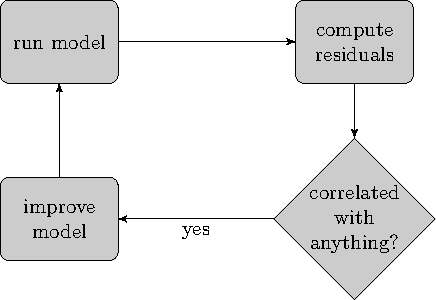
\includegraphics[width=0.7\textwidth]{09-privacy/PredictionWeb_tikz_welcome.pdf}}
\else 
\fi 
\caption{A highly stylized depiction of ongoing analytical model improvement.}
\label{fig:process}
\end{figure}

To emphasize the role of real and perceived risks, I will assume, this time, that you run a large global company with realtime operations assisted in some material way by predictive analytics. Quite possibly you have invested vast sums of money in combinations of people and machines that provide thousands, millions or billions of short term predictions. 

The engines that drive your profit and loss might literally be engines. Or they might be intelligent applications advancing sales, trading, navigation, recruitment or customer satisfaction. Inside these engines is a common ingredient: bespoke repeated prediction. Those predictions are created by data scientists you employ. They try to gather relevant models and data. 

Because your bottom line is driven by an intelligent application of some flavor, and because that is in turn driven by repeated short term prediction, a highly stylized depiction of your company's never ending quest is presented in Figure \ref{fig:process}. 

Of course no prediction is perfect. The difference between your model predictions and the revealed truth is computed every time. By this means you produce a flood of individual ex-post model residuals. You search for 
data sources or new transformations of existing data that are correlated to these residuals.  

If your employees find a new well motivated statistical relationship, you might include the features in your model. The process repeats. The spend never ends. There may be no absolute, or even relative notion of what you are getting for your money. 



\section{The oracle arrives}

One day you are presented with something that seems like a free option. It is touted as a mysterious source of predictive power. It exists inside your company's firewall, and can be used in a variety of simple ways. 

This particular oracle operates in conversational style. You send it a question and it provides a prediction. You hope it will help you speed the cycle in Figure \ref{fig:process}. You could, it occurs to you, see if the oracle can predict your model residuals (which by definition you can not). 

What's not to love? Well, one concern is privacy. You are told that this oracle invites machines and people to predict your data. That is why it is so effective, and constantly improving. The marginal cost for an algorithm to attack your data stream is close to zero, since it was designed to address several other problems as well. No human involvement is required.  

As it happens, you do not consider your model residuals to be highly proprietary. Nobody is likely to reverse their meaning and nobody has your model. You can send only a subset of residuals and, as a kicker, you are assured by experts in privacy preserving machine learning that nobody will ever recover your residuals (even if they were to care about them, which is unlikely). 

Indeed nobody will learn {\em anything} about these numbers, even statistically speaking. And yet this oracle will allow you to benefit from both data and models in the outside world that you might not otherwise discover. 

So you give it a spin. For a while the oracle returns a sequence of zeros. You've told it that you are sending model residuals. It cannot determine with any confidence that zero is not its best estimate of your model residuals, so it merely returns zero. You shrug, but there is no harm done. 


But then one day the oracle starts returning small numbers. It does not do this for every prediction. Most are still zeros, but just a few are not. Over time the numbers get slightly larger and the number of zeros fewer yet.  


The oracle, whose construction you will learn about only later, is trying to identify the statistical bias in each and every prediction your model is making. The oracle does not predict the entirety of your errors - to do so would be to imply perfect prediction. However, by subtracting the numbers the oracle returns to you from your existing model predictions, you are able to create a new prediction that reduces the error.  

Well you say, isn't that something? But the world is full of spurious correlations.\footnote{\cite{spurious}} For a while, you and your team are skeptical whether the oracle's performance will continue to be strong. 


Sensibly, you limit the use to cases where thousands or tens of thousands of predictions are made daily, in order to reduce the likelihood that the oracle's apparent prescience is a ruse. You steer away from asking the oracle for long term predictions of singular events, most commonly associated with the world ``prediction.'' 

You don't try to use the oracle to generate ``alpha'' - excess returns in the stock market. You focus on the bespoke predictions that help your business.  The oracle continues to perform. Day after day. In fact, it gets even more accurate. 

\section{Tentative steps}

This is your first introduction to the prediction web, whether you realize it or not. Only later you will discover that the search performed by this oracle is not miraculous but merely basic economics, and that you have tapped into a collective statistical construction that will one day power {\em all} AI applications - in one way or another. You are using it without taking on any real business risk.       

But for now you are still skeptical. You are not prepared to throw out your model and rest entirely on the oracle for realtime business decisions without knowledge of its inner workings. You receive pushback from compliance, dampening your enthusiasm. Is it worth it? 

Meanwhile, you're making yourself unpopular with some data scientists and some managers of data scientists. They mention privacy a lot but what they are really thinking is {\em oh Lord, this is a potential mark-to-market event for my skill set and my entire group}. You ask your quants to explain why their model residuals are proprietary - as compared with merely being closely guarded. 

They go quiet, but drag their feet. Sending your residuals out for inspection feels a bit too much like posting a stool sample to a cancer screening company. You know you should do it, but you are fearful of the results. 

The oracle is unperturbed by the machinations of your company. It simply keeps doing its job. The length of the time-series you have created keeps growing. The history is more informative. Unbeknownst to you, it is patiently discovering new sources of data, new transformations of that data, and new approaches to processing it, storing it and of course, applying advanced mathematical models to it. 

It's tentacles - the graph of computation performed by disparate micro-managers behind the scenes - stretch outward from the other side of the oracle. They reach transport data, financial data and the internet of things. They use data sources you will never know about, or never need to.   

You revisit your concerns. It occurs to you that because you have focused on streaming prediction problems the risk is reduced substantially. Both the economic benefit and downside accumulates over thousands or millions of decisions, each one of manageable size. 

So you create a hybrid. You enforce a rule stating that the prediction you use will always lie within a fixed distance from an approved in-house model. This amounts to bounding the residual thresholds. Since very few predictions trigger this rule, you retain ninety five percent of the economic benefit, while ensuring that any increase in your economic risk is immaterial. 


\section{Infection}

Slowly, the prediction web begins to worm its way into every aspect of your operations. You migrate some of the intelligence behind the oracle into your model. By using the oracle you become aware of a source of data you never imagined would help you. After carefully incorporating the new source, the oracle's residual estimates go down. 

This proves to be rather addictive, yet you hunger for a faster process, one freed of the limitations of your quantitative practices. Your engineers start to implement some hooks behind the oracle adding new levels of functionality without jeopardizing your data privacy. You are now able to ask the oracle for predictions of data you supply it going well beyond your starting pattern: the use of model residuals only.  

You become more confident in the underlying technology and begin to ask the oracle to predict things for which you have no existing model. The instrumentation of your business comprises a collection of numbers intended to provide up to the minute information deemed critical. You realize that any such number, produced for your benefit at some cost already, can be enhanced with a forward looking estimate of the very same number for almost no additional cost on the margin.

Still later, you examine the inner working of your decision making algorithms powered by control theory and reinforcement learning methods. You identify various points in these calculations where a parameter is set using the minimization or maximization of some predictive criterion.

You start to incorporate oracles into darker places such as intermediate value function calculations used to navigate, set prices and solve logistic problems on the fly. You start to outperform your competitors because the brain that powers your business is an analytical supply chain. Every step in the chain is constantly improving.  

Whether you realize it fully or not, you are finally free of the most important limitation of your existing practices - the models were comprehensible to a single person, and thereby constrained by human cognitive capability. 

Your business is now powered by something far more potent - a global prediction web that sees more and more exogenous data every day, and whose artificial fauna match every conceivable algorithm to the specific task you have at hand.  

And it costs you next to nothing. 

Indeed, sometimes you get paid. It turns out that one sequence of true data points you need predicted is valuable to somebody else's prediction capability. Sometimes, the economic value of the data you inject into the grid exceeds the rapidly falling cost of bespoke prediction you have called upon the oracle to perform. 

You are being rewarded in a small way for helping to solve the modern day tragedy of the commons - the lack of an extant realtime feature space usable by anyone, including companies much smaller than your own. 

Unbeknownst to you, independent cinemas, bakeries, non-profits and individuals are contributing tiny amounts of money, or eyeballs, to the same prediction web you use. Algorithms automatically resuse themselves. The power of data is automatically shared. 

Next you contribute a model. Some non-proprietary feature generator that one of your data scientists had open sourced grows legs. It navigates across the prediction web, on its own, and finds a dozen places where it adds value. 

In the process, other algorithms analyze it and assess its relative worth in different situations. The additional experience suggests improvements. You discover that when contributing to the open source community, you get back more than you put in. 


You and your company are now part of the prediction web in every sense. You are contributing to a collective solution to the {\em almost} intractable problem of search in the space of models and data, at least as it applies to 
optimization of real-time business processes. You will be entangled, now, and for as long as you operate. And so will everyone else in your industry, sooner or later. 